\chapter{Results and Discussion}\label{chap:results}
% Evaluation Criteria:
% - Quality of explanation (written)
% - Support with diagrams, tables and figures
% - Table headings and figure captions
% - Clear axis labels on all figures
% - Figure complexity
% Discussion
% - Quality of explanations (written)
% - Comparison with related work
% - Discussion of implications
% - Discussion of limitations

\begin{figure}[!htbp]
    \begin{centering}
        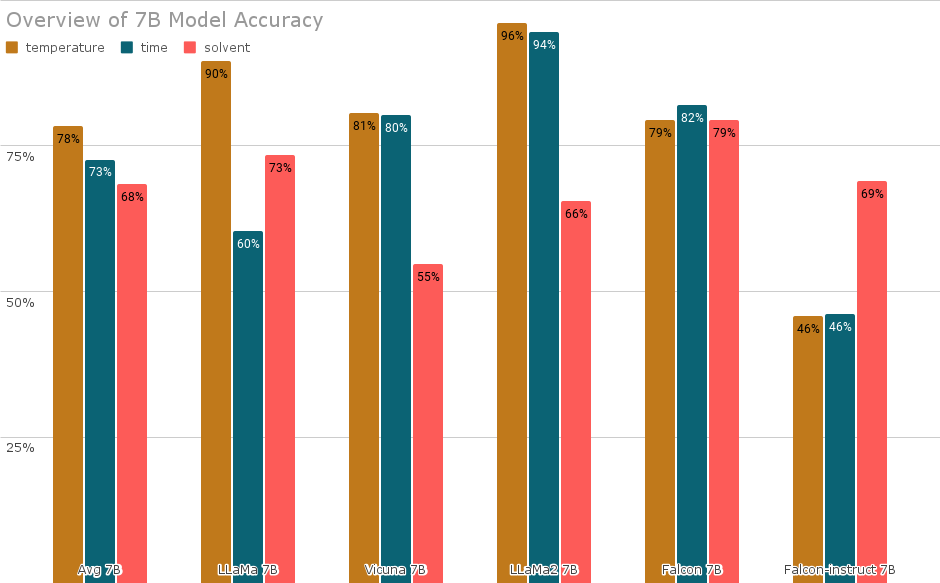
\includegraphics[width=0.9\textwidth]{img/overview_7b_accuracy}
        \caption[Overview of 7B Models Accuracy]{\textbf{Overview of the Accuracy of Models with a Size of 7B parameters.}
        On the left is the average over all 7B sized models.
        The accuracy of \ttemp and \ttime is within 3 \glspl{pp} of the other for each model except \model{llama}, where the difference is 30 \glspl{pp}.
        On average, the accuracy for \ttemp is 78\%, 73\% for \ttime, and 68\% for \tsolv.
        }
        \label{fig:7b_acc}
    \end{centering}
\end{figure}


\begin{figure}[!htbp]
    \begin{centering}
        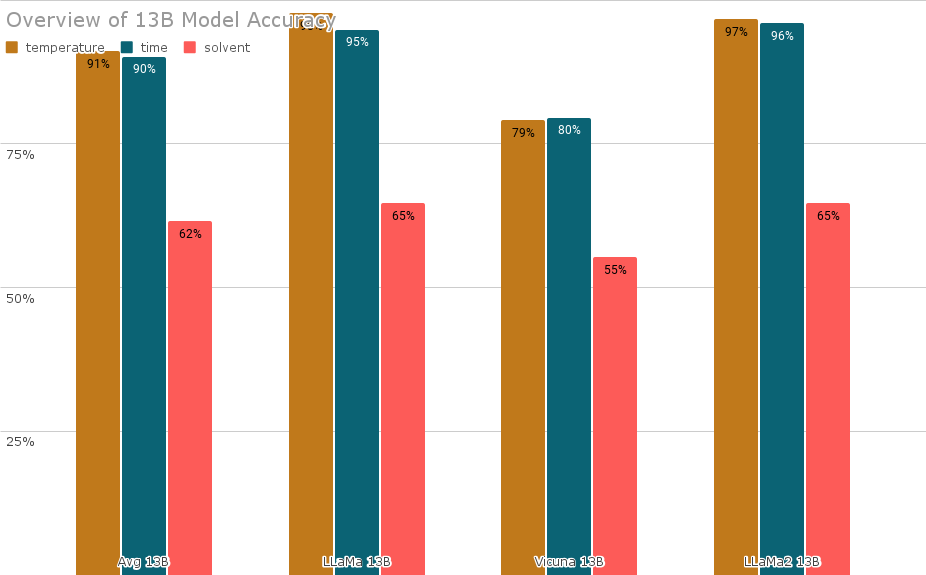
\includegraphics[width=0.9\textwidth]{img/overview_13b_accuracy}
        \caption[Overview of 13B Models Accuracy]{\textbf{Overview of the Accuracy of Models with a Size of 13B parameters.}
        Leftmost is the average over all 13B sized models.
        \model{falcon} does not have a 13B sized variant.
        On average, the accuracy for \ttemp is 90.3\%, 89.1\% for \ttime and 54.4\% for \tsolv.
        }
        \label{fig:13b_acc}
    \end{centering}
\end{figure}


\begin{figure}[!htbp]
    \begin{centering}
        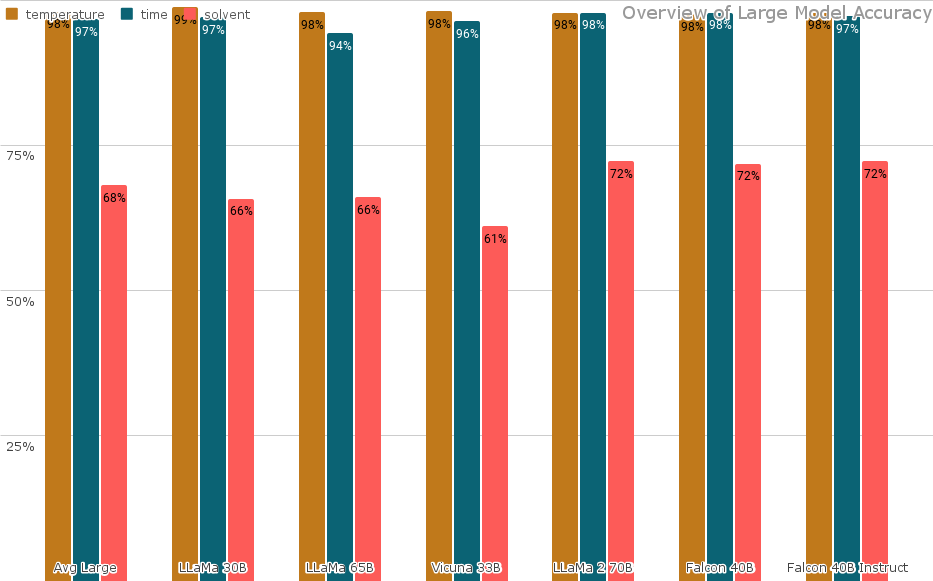
\includegraphics[width=0.9\textwidth]{img/overview_large_accuracy}
        \caption[Overview of Large Model Accuracy]{\textbf{Overview of the Accuracy of Models with a Size over 30B parameters.}
        Leftmost is the average over all models upwards of 30B parameters.
        On average, the accuracy for \ttemp is 98\%, 97\% for \ttime and 68\% for \tsolv.
        \model{llama2} does not have a 30B or 33B-sized variant.
        There is also no \model{vicuna}-65B variant made available from \gls{lmsys}.
        \model{llama2} and both \model{falcon} models achieve 72\% accuracy on \tsolv extraction, 6-11 \glspl{pp} more than other models.
        }
        \label{fig:large_acc}
    \end{centering}
\end{figure}


\section{7B Parameter Models}\label{sec:result:7b}
As can be seen in \figref{7b_acc}, most models achieve decent accuracies in extracting \ttemp and \ttime data.
Most models hover just below 60\% in \tsolv accuracy, with \model{vicuna} being an outlier, achieving an accuracy of only 27\%.
\todo{build graph of unit mistakes}

\section{13B Parameter Models}\label{sec:result:13b}
See \figref{13b_acc}. 
\model{vicuna} substantially improved its \tsolv accuracy compared to its 7B variant, where it is now only 10 \glspl{pp} behind \model{llama} and \model{llama2}.
\model{vicuna} 13B is also the weakest in accuracy for \ttemp and \ttime, trailing by about 14 \glspl{pp}.

\section{Large Models}\label{sec:result:large}
See \figref{large_acc}. As much as scores between models differ in \secref{result:7b}, differences between large models are marginal at best

\section{Discussion}\label{sec:discussion}
\todo{what does it all mean}


% \verb!2023-09-09 16:05:36 ERROR    pcp: Could not find `cid` for [distilled H2O]!

